


On official CFP-FP pairs, raw TAR increases from 87.71\% for MobileFaceNet to 94.89\% for ResNet50 at the 0.1\% training-FAR target. Both have observed test FAR 0.143\%. Table~\ref{tab:encoder-cfp} reports the separate screened-subset comparison. Protected TAR rises for every method and length: from \MbfSmallTar{} to \RnetSmallTar{} at 128 bits, and from \MbfLargeTar{} to \RnetLargeTar{} at 512 bits.

Higher utility does not remove the tested reconstruction vulnerability. At ten exposures, MobileFaceNet calibrated cross-image fresh-key ASR is \MbfSmallAsr{} at 128 bits and \MbfLargeAsr{} at 512 bits. The corresponding ResNet50 ranges are \RnetSmallAsr{} and \RnetLargeAsr{}. All six paired ResNet50-minus-MobileFaceNet ASR intervals lie above zero. These pointwise intervals resample the 195 unique test identities while retaining dependencies across overlapping splits and keys; they condition on the fitted models and thresholds. They do not establish that every stronger encoder is less secure.

Fresh-key acceptance and reconstruction cosine do not improve in parallel. For 128-bit RO and SRHT, exposed-image cosine stays near 0.81 with either encoder, although acceptance rises with ResNet50. All three 512-bit ResNet50 configurations also admit high acceptance. Thus, stronger genuine recognition cannot be taken as evidence that the protected representation better resists known-operator reconstruction.

Table~\ref{tab:encoder-lfw} gives the corresponding LFW recognition extension. Raw matcher-only TAR changes from 98.66\% to 99.03\%. At 128 bits, ResNet50 TAR is 92.28\% for RO, 92.10\% for SRHT, and 94.66\% for PCA-guided RO, compared with 82.99\%, 84.48\%, and 85.22\% for MobileFaceNet. These recognition results extend the utility comparison; they do not extend the LFW attack evidence.

\begin{table*}[t]
\caption{Matched encoder comparison on screened CFP. Rates are percentages; ASR differences are percentage points.}
\label{tab:encoder-cfp}\centering\footnotesize
\begin{tabular}{@{}rlrrrrr@{}}\toprule
Bits & Method & MBF TAR / FAR & R50 TAR / FAR & MBF ASR & R50 ASR & ASR difference [95\% CI]\\\midrule
128 & RO & 39.33 / 0.134 & 65.50 / 0.133 & 19.66 & 38.46 & 18.80 [16.68, 20.86]\\
128 & SRHT & 37.76 / 0.113 & 65.12 / 0.120 & 18.84 & 38.28 & 19.43 [17.03, 21.81]\\
128 & PCA-guided RO & 43.50 / 0.115 & 66.94 / 0.103 & 32.96 & 53.09 & 20.13 [17.74, 22.68]\\
512 & RO & 82.52 / 0.172 & 94.61 / 0.134 & 78.02 & 92.30 & 14.28 [11.13, 17.52]\\
512 & SRHT & 81.95 / 0.167 & 94.67 / 0.128 & 77.52 & 92.23 & 14.71 [11.67, 17.95]\\
512 & PCA-guided RO & 82.38 / 0.200 & 94.37 / 0.130 & 78.56 & 92.03 & 13.48 [10.34, 16.72]\\
\bottomrule\end{tabular}
\tabnote{MBF: MobileFaceNet; R50: ResNet50 ArcFace. Each encoder has a separate validation-only threshold targeting 0.1\% FAR. ASR is calibrated cross-image fresh-key acceptance at $K=10$. The fresh operator is hidden from reconstruction. Paired percentile intervals use 2000 identity resamples and condition on the fitted pipelines; they are pointwise and not multiplicity-adjusted. These replication runs remain separate from the original baseline tables.}
\end{table*}

\begin{table}[t]
\centering
\caption{LFW official-pair recognition: encoder comparison.}
\label{tab:encoder-lfw}
\small
\begin{tabular}{lrrrr}
\toprule
& \multicolumn{2}{c}{TAR (\%)} & \multicolumn{2}{c}{FAR (\%)} \\
Method & MBF & R50 & MBF & R50 \\
\midrule
Raw & 98.66 & 99.03 & 0.101 & 0.101 \\
RO & 82.99 & 92.28 & 0.094 & 0.080 \\
SRHT & 84.48 & 92.10 & 0.094 & 0.094 \\
PCA-guided RO & 85.22 & 94.66 & 0.087 & 0.094 \\
\bottomrule
\end{tabular}
\tabnote{Matcher-only evaluation uses 5965 valid pairs, with thresholds fitted on the other nine folds at a 0.1\% FAR target. Protected templates have 128 bits; rates average five fixed keys. MBF: MobileFaceNet; R50: ResNet50 ArcFace. The full 6000-pair operational results are retained in the evidence. Fold-specific PCA excludes held-out identities from fitting.}
\end{table}


\begin{figure*}[!t]
\centering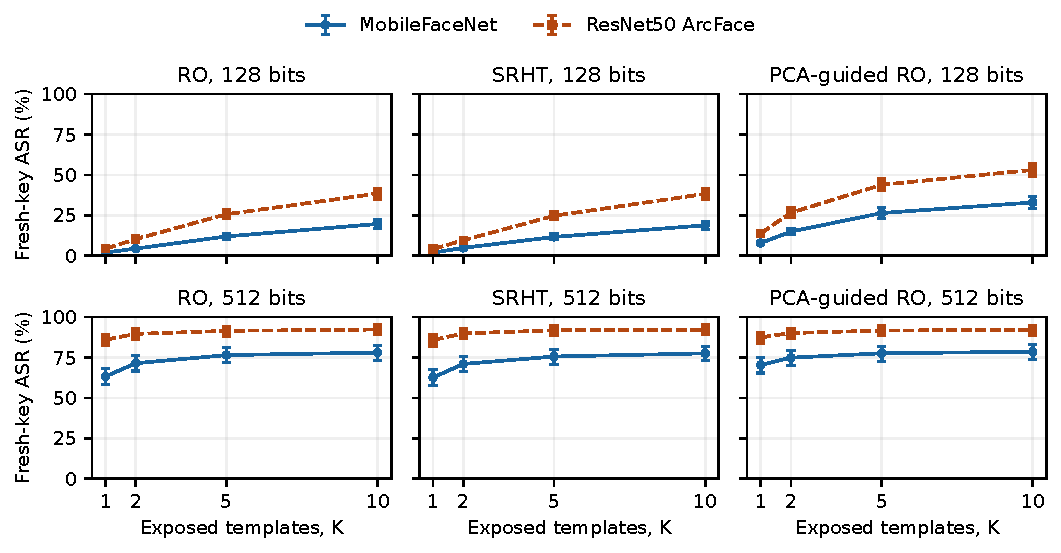
\includegraphics[width=0.92\textwidth]{encoder_exposure.pdf}
\caption{CFP encoder replication: calibrated cross-image fresh-key ASR over exposure count at 128 bits (top) and 512 bits (bottom). Error bars show pointwise conditional 95\% identity-bootstrap intervals. Both encoders use identical screened crops and exposure schedules, with separately fitted models and validation-only thresholds.}
\label{fig:encoder-exposure}
\fignote{The stronger recognition checkpoint still permits substantial fresh-key attack acceptance.}
\end{figure*}


Unchanged old CFP records continue to have low cross-image replay acceptance. Across the two encoders, three methods, and two directions, mean transition rates are approximately 0.038--0.076\% at 128 bits and 0.004--0.013\% at 512 bits. Template-only linkage with ten records has trained-score AUC 0.530--0.542 at 128 bits and 0.559--0.567 at 512 bits. These descriptive outcomes concern the tested classifier and fixed key schedule; they do not prove unlinkability or resistance to a stronger attacker.

The replication reports conditional intervals at validation-FAR targets $10^{-4}$, $10^{-3}$, and $10^{-2}$, together with a descriptive threshold sweep and measured test FAR alongside TAR and ASR. Complete exposure curves, paired contrasts, and threshold plots are retained in the accompanying results. Lower attack acceptance under stricter matching must be read alongside increased genuine rejection. The hidden fresh operator and digital embedding-input interface remain unchanged.


Figures~\ref{fig:cfp-recognition} and~\ref{fig:lfw-recognition} present recognition separately for the screened CFP protocol and official LFW pairs. CFP intervals quantify conditional identity variation; LFW error bars describe variation across five fixed keys and are not confidence intervals. The two uncertainty summaries must not be conflated.

Figure~\ref{fig:paired-encoder} reports paired differences directly. At the primary validation target, all six protected-recognition contrasts and all six calibrated ten-exposure ASR contrasts favor higher acceptance with ResNet50. Figure~\ref{fig:paired-exposure} shows that all twelve calibrated exposure-growth intervals are positive. These pointwise results quantify consistency across the tested configurations without providing simultaneous family-wise coverage.

Figure~\ref{fig:reconstruction-quality} distinguishes recovery of the exposed image's embedding from transfer to a different photograph of the same identity. These endpoints capture source fidelity and cross-image identity information, respectively. Neither substitutes for the fresh-key acceptance test, whose outcome also depends on the transformation and threshold.

\begin{figure}[!tb]
\centering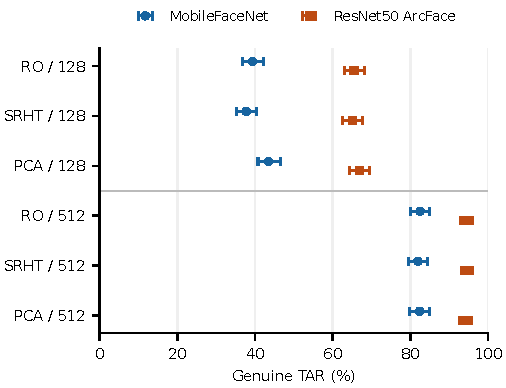
\includegraphics[width=\columnwidth]{cfp_recognition_ci.pdf}
\caption{Protected genuine recognition on screened CFP at the $10^{-3}$ validation-FAR target. Error bars are pointwise conditional 95\% identity-bootstrap intervals.}
\label{fig:cfp-recognition}\fignote{Matched inputs and protocols use encoder-specific fits and thresholds; PCA denotes PCA-guided RO, and row suffixes give bit lengths.}
\end{figure}
\begin{figure}[!tb]
\centering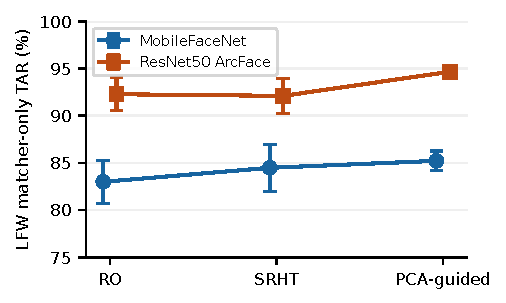
\includegraphics[width=\columnwidth]{lfw_recognition_sd.pdf}
\caption{LFW matcher-only recognition at 128 bits under official folds. Error bars show one standard deviation across five keys, not confidence intervals.}
\label{fig:lfw-recognition}\fignote{This extension evaluates recognition; it does not provide a second-encoder LFW attack result.}
\end{figure}
\begin{figure}[!tb]
\centering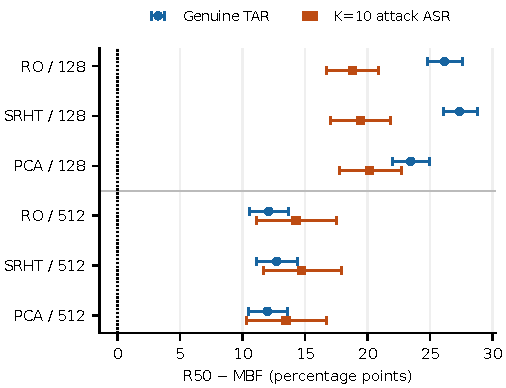
\includegraphics[width=\columnwidth]{paired_encoder_effects.pdf}
\caption{Paired ResNet50-minus-MobileFaceNet differences in genuine TAR and calibrated fresh-key ASR at $K=10$. Bars show pointwise conditional 95\% intervals; the dotted line marks zero.}
\label{fig:paired-encoder}\fignote{Positive differences mean higher acceptance, which has different implications for genuine and attack inputs.}
\end{figure}
\begin{figure}[!tb]
\centering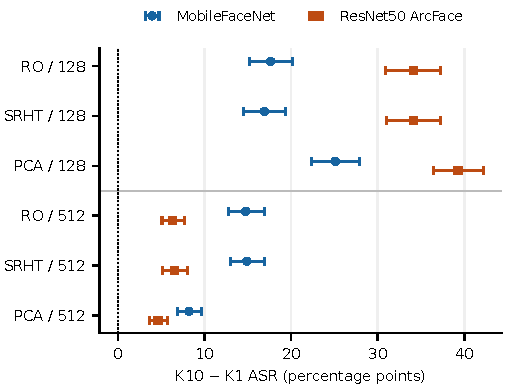
\includegraphics[width=\columnwidth]{paired_exposure_effects.pdf}
\caption{Paired $K=10$ minus $K=1$ calibrated fresh-key ASR differences for screened CFP. Bars show pointwise conditional 95\% intervals at the $10^{-3}$ validation-FAR target.}
\label{fig:paired-exposure}\fignote{Every plotted interval lies above zero; trials sharing an identity retain common bootstrap weights.}
\end{figure}
\begin{figure*}[!t]
\centering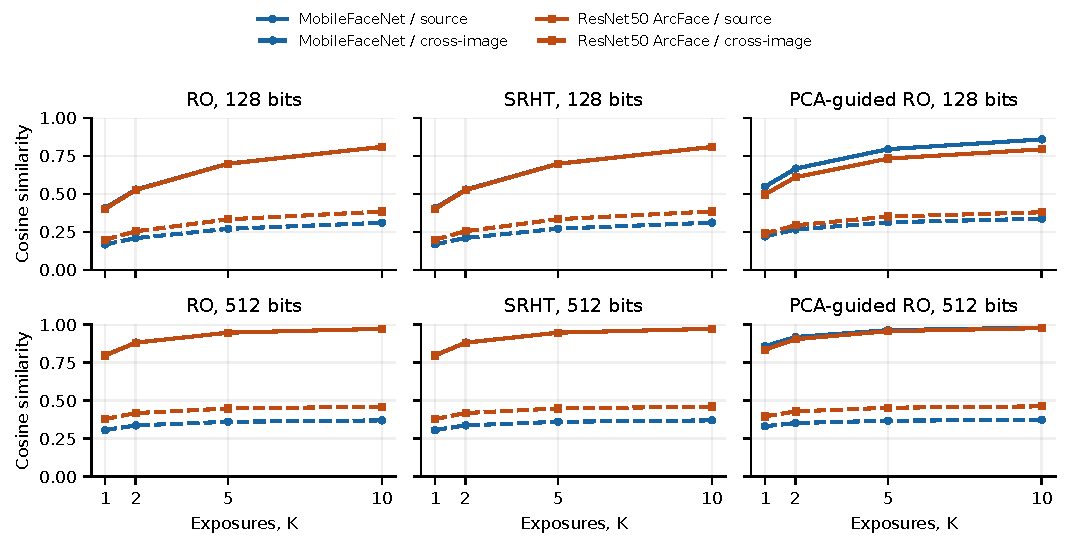
\includegraphics[width=.97\textwidth]{reconstruction_quality.pdf}
\caption{Calibrated reconstruction cosine over exposure count on screened CFP. Color identifies the encoder; solid and dashed lines distinguish the exposed source from the cross-image reference.}
\label{fig:reconstruction-quality}\fignote{Lines show point estimates, not uncertainty bands; cosine is unitless and is not attack acceptance.}
\end{figure*}
\begin{figure}[!tb]
\centering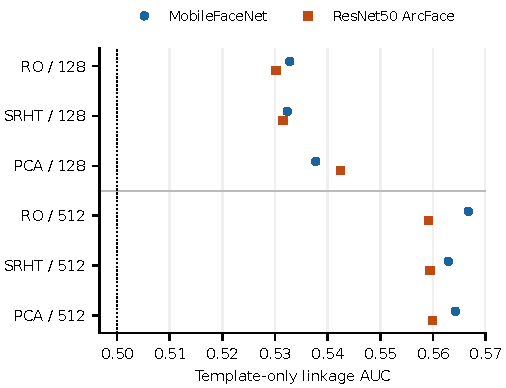
\includegraphics[width=\columnwidth]{linkage_comparison.pdf}
\caption{Template-only linkage at $K=10$ in the matched CFP replication. The dotted line denotes chance AUC; these descriptive means have no added confidence intervals.}
\label{fig:linkage-enc}\fignote{The learned score shows limited discrimination under this access model, which excludes old operators.}
\end{figure}

Figure~\ref{fig:linkage-enc} complements the inversion results with the template-only attacker. Figures~\ref{fig:enc-target128} and~\ref{fig:enc-target512} show how validation targets alter genuine acceptance, test FAR, and attack acceptance. At target $10^{-4}$, calibrated 512-bit $K=10$ ASR remains 69.59--70.54\% for MobileFaceNet and 89.01--90.09\% for ResNet50. These values belong to the matched replication, distinct from the original MobileFaceNet sweep. The stricter target reduces attack acceptance without demonstrating population FAR control at $10^{-4}$.
\begin{figure*}[!t]
\centering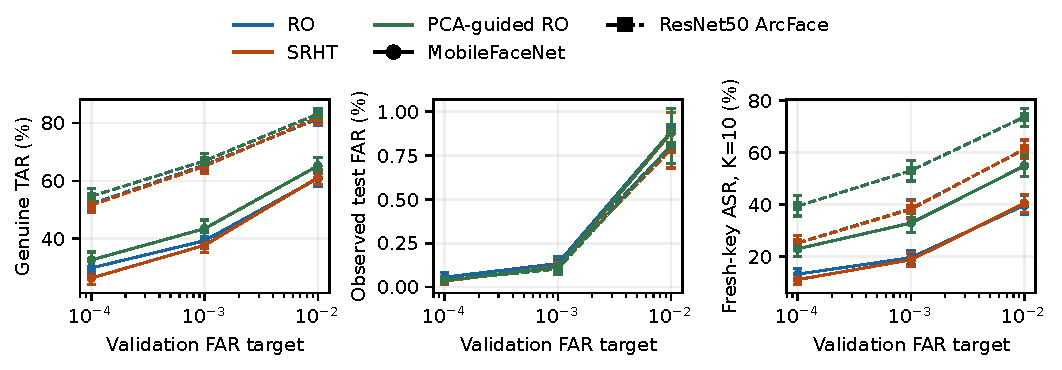
\includegraphics[width=\textwidth]{encoder_threshold_targets_128.pdf}
\caption{Matched CFP sensitivity at 128 bits: genuine TAR, observed test FAR, and calibrated $K=10$ fresh-key ASR at three validation-FAR targets. Error bars show pointwise conditional 95\% intervals.}
\label{fig:enc-target128}\fignote{Validation targets set the thresholds; the middle panel reports the separately observed test FAR.}
\end{figure*}
\begin{figure*}[!t]
\centering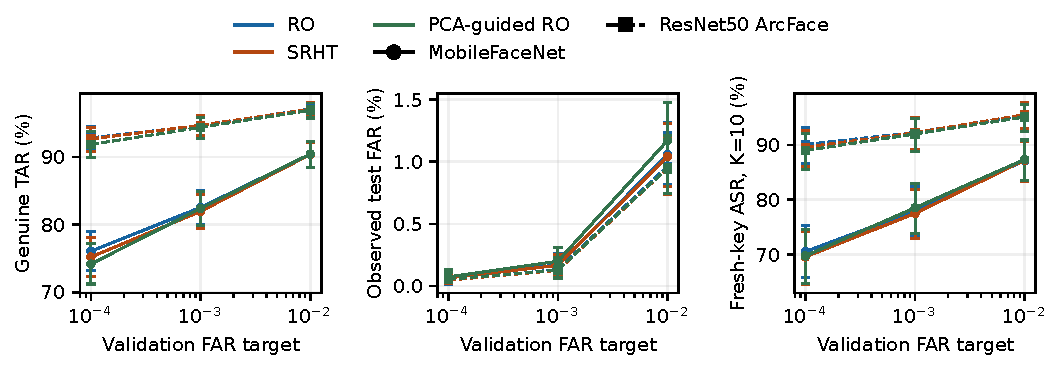
\includegraphics[width=\textwidth]{encoder_threshold_targets_512.pdf}
\caption{Matched CFP sensitivity at 512 bits with the same endpoints and validation-target convention as Fig.~\ref{fig:enc-target128}. Error bars show pointwise conditional 95\% intervals.}
\label{fig:enc-target512}\fignote{Substantial attack acceptance persists at the strictest evaluated validation target.}
\end{figure*}
